\documentclass{article}
\usepackage{a4wide}
\usepackage{norsk}
\usepackage{amsmath}
\usepackage{amssymb}
\usepackage{dsfont}
%\usepackage[dvips]{epsfig}
%\usepackage{graphicx}
\usepackage{fancyhdr}
\usepackage{listings}
\usepackage{nomencl}
\usepackage[pdftex]{graphicx}

\pagestyle{fancy}
\lhead{\footnotesize \parbox{11cm}{Andreas Johann H\"ormer (753179)}}
\rhead{\footnotesize {Laboratory 1}}
\chead{\footnotesize {TTT4170}}

\title{Report Room acoustics (Lab 1)}
\author{Andreas Johann H\"ormer}
\date{14.02.2014}

\begin{document}

\maketitle
%\\[5cm]
\begin{center}
TTT4170 Audio Technology\\[3cm]
Lab group:
\begin{itemize}
\item Andreas Johann H\"ormer
\item Milan Stojkovic
\item y\\[3cm]
\end{itemize}
Report delivered: 27.02.2014\\[6cm]
FACULTY OF INFORMATION TECHNOLOGY, MATHEMATICS AND ELECTRICAL ENGINEERING\\
NORWEGIAN UNIVERSITY OF SCIENCE AND TECHNOLOGY
\end{center}

\tableofcontents

\newpage
\section{Summary}

\newpage
\section{Introduction}
This laboratory exercises treated different measurement and calculation methods of room acoustics. Therefore the dimensions of a room are measured and reverbation times at different octave bands and sound pressure levels as function of distance to the sound source are calculated. Sabine's formula is used for calculations. Further the hall radius in the room and absorption coefficients at different frequency bands are calculated.\\
Measurements were done in the lecture room EL2 in Elbygget of NTNU. The dimensions of the room were measured with a BOSCH laser meter and rounded to the next meter. The room is 10m width and 10m long, the ceiling is 4m in the front and 3m in the back. The floor is 3.4m horizontal and has a slope starting at 3.4m to the end at 10m. The floor is linoleum, at the slope there are chairs. On the backside there are some absorbers, the left side is gypsum, at the right side of the lecture hall are mostly glass areas (windows). In the front there is a wooden blackboard at the wall, the ceiling is gypsum. EL2 has a volume of $V=367m^3$ and a surface area of $S=344m^2$. The calculation can be found in chapter \ref{sec:roomparam}.

\section{Measurements}
\subsection{Equipment}
The measurements were done with a notebook and WinLMS-Software. A measurement microphone was put on a microphone stand. As sound source a loudspeaker (which is assumed as omnidirectional) was used.
\subsection{Reverbation time}
\subsubsection{Method}
For measuring the reverbation time of the room the microphone was placed at three different positions. One was chosen in the back of the room, one in the middle and one in a corner in the front. The exact positions in the lecture room can be found in table \ref{tab:revmeasure}. The measurements were done with a swept sine with starting frequency 50Hz to an end frequency of 20kHz. This is done in every measurement point, then the results are averaged.
\begin{table}
\begin{center}
\begin{tabular}{|c c|}
\hline
\includegraphics[width=6cm,keepaspectratio=true]{frontpic} & 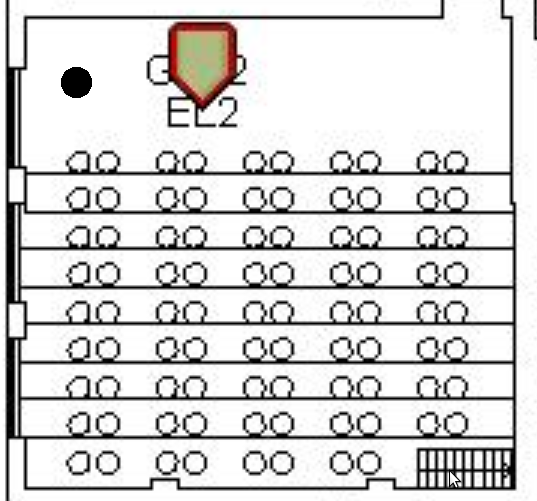
\includegraphics[width=5cm,keepaspectratio=true]{front}\\
\multicolumn{2}{|c|}{measurement in the left front corner}\\
\hline
\includegraphics[width=6cm,keepaspectratio=true]{middlepic} & 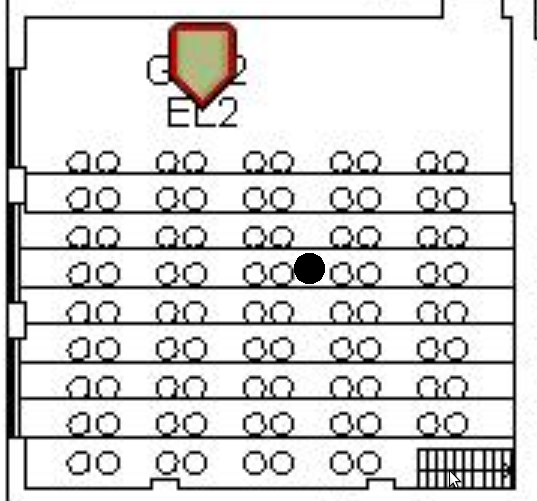
\includegraphics[width=5cm,keepaspectratio=true]{middle}\\
\multicolumn{2}{|c|}{measurement in the middle of the room}\\
\hline
\includegraphics[width=6cm,keepaspectratio=true]{backpic} & 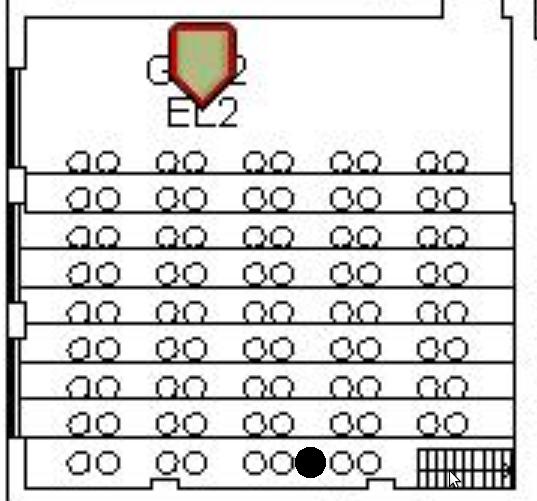
\includegraphics[width=5cm,keepaspectratio=true]{back}\\
\multicolumn{2}{|c|}{measurement at the backside}\\
\hline
\end{tabular}
\caption{microphone positions}
\label{tab:revmeasure}
\end{center}
\end{table}
\subsubsection{Results}
The reverbation time was analyzed with WinLMS and an average has been calculated with
$$T_{60,avg}=\frac{T_{60,front}+T_{60,middle}+T_{60,back}}{3}$$
The values for the reverbation times and the averages are listed in table \ref{tab:Tmeasurements}. Here one special result can be obtained. The reverbation time for the octave band $125Hz$ is much longer than for the other octave bands. One further measurement result is worth mentioning. At the front corner the reverbation time at $250Hz$ is very low. This can be caused due to negative interference at the microphone position. The measurement results from WinLMS are listed in figures \ref{fig:reverbationfront}, \ref{fig:reverbationmiddle} and \ref{fig:reverbationback}. The plots show that at low frequencies the reverbation times differ very much. This is because of the large wavelength. The amplitudes at the microphones differ very much, so the reverbation times differ much too. Generally it can be obtained that the reverbation times are decreasing slightly with increasing frequency.
\begin{table}
\begin{center}
\begin{tabular}{|c||c|c|c||c|}
\hline
octave band & back & middle & front & average	\\
$Hz$		&	$s$	&	$s$		&	$s$		&	$s$		\\
\hline
\hline
125			& 1.34	&	0.98	&	1.58	&	1.3		\\
\hline
250			& 0.86	&	0.72	&	0.07	&	0.55	\\
\hline
500			& 0.75	& 	0.78	&	0.49	&	0.67	\\
\hline
1k			& 0.73	&	0.72	&	0.72	&	0.72	\\
\hline
2k			& 0.75	&	0.78	&	0.78	&	0.77	\\
\hline
4k			& 0.64	&	0.63	&	0.65	& 	0.64	\\
\hline
\end{tabular}
\caption{$T_{60}$ measurements and average}
\label{tab:Tmeasurements}
\end{center}
\end{table}
\begin{figure}[htbp]
\begin{center}
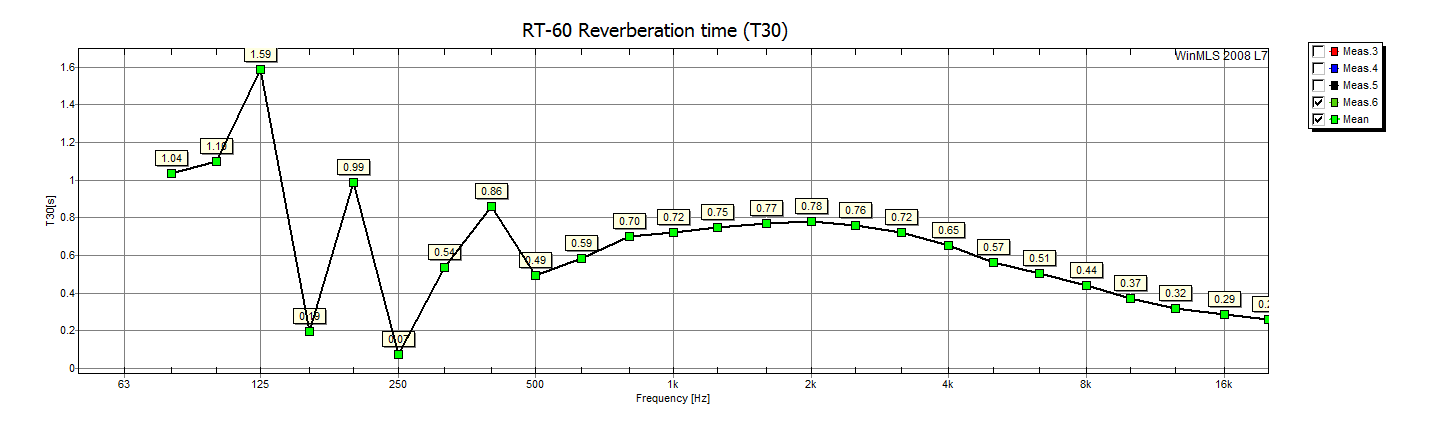
\includegraphics[width=15cm,keepaspectratio=true]{reverbationfront}
\caption{reverbation time in the front position}
\label{fig:reverbationfront}
\end{center}
\end{figure}
\begin{figure}[htbp]
\begin{center}
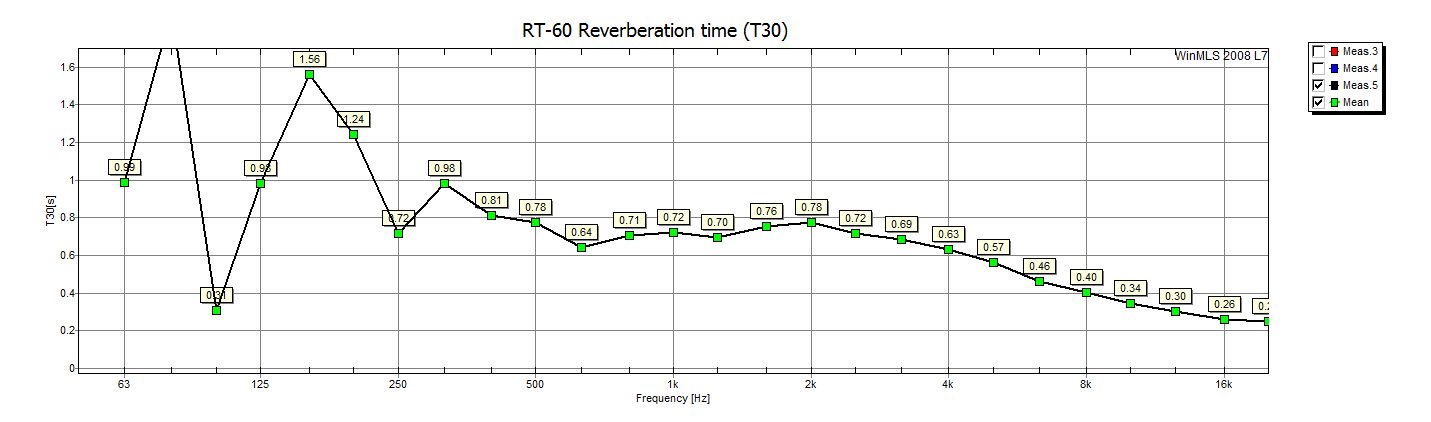
\includegraphics[width=15cm,keepaspectratio=true]{reverbationmiddle}
\caption{reverbation time in the middle position}
\label{fig:reverbationmiddle}
\end{center}
\end{figure}
\begin{figure}[htbp]
\begin{center}
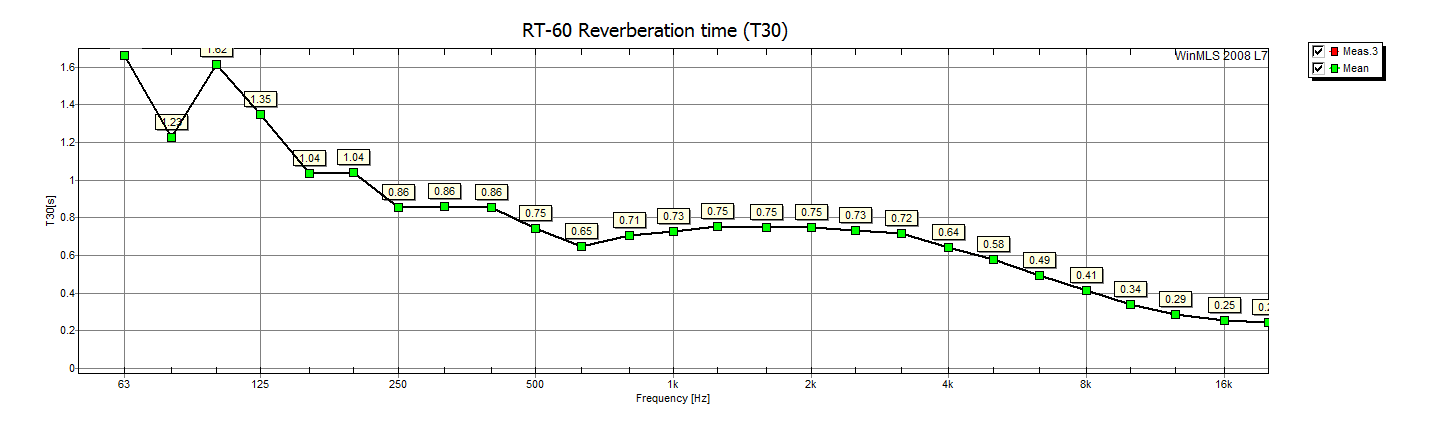
\includegraphics[width=15cm,keepaspectratio=true]{reverbationback}
\caption{reverbation time in the back position}
\label{fig:reverbationback}
\end{center}
\end{figure}
\subsection{Sound pressure level}
\subsubsection{Method}
\subsubsection{Results}
\begin{figure}[htbp]
\begin{center}
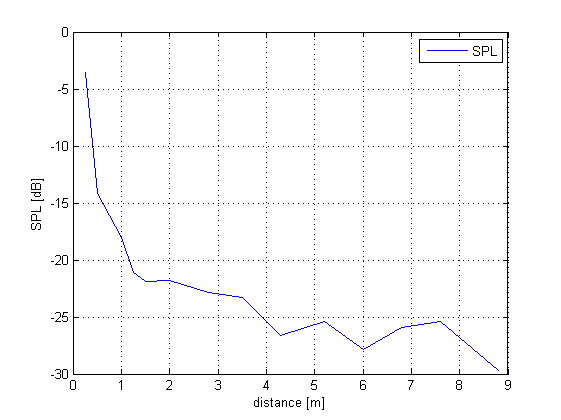
\includegraphics[width=10cm,keepaspectratio=true]{SPL}
\caption{Sound Pressure Level as function of distance}
\label{fig:spl}
\end{center}
\end{figure}

\newpage
\section{Calculations}

\newpage
\section{Conclusion}

\newpage
\section{Appendix}
\subsection{Calculation of room parameters\label{sec:roomparam}}
\subsubsection{room volume}
The room volume can be calculated by calculating the room as whole cuboid and subtracting the volume below the slope.
\begin{equation}
V=V_{total}-V_{below\,slope}
\end{equation}
$$V=10m\cdot 4m\cdot 10m-\frac{6.6m\cdot 1m\cdot 10m}{2}$$
$$V=367m^3$$
\subsubsection{surface area}
\begin{equation}
S=S_{ceiling}+S_{floor}+S_{slope}+S_{front}+S_{back}+2\cdot S_{wall}
\end{equation}
$S_{ceiling}$ covers whole area above the lecture room, $S_{floor}$ defines the horizontal floor area. $S_{slope}$ covers all area on the slope, mainly the area where the chairs are in the room. The wall surface $S_{wall}$ is everything on the left and right side of the lecture hall. At this area the surface area below the slope has to be subtracted. $S_{front}$ and $S_{back}$ cover the front and the back part of the wall.\\
So the total surface area is
$$S=10m\cdot\sqrt{6.6^2m^2+1^2m^2}+3.4m\cdot 10m+10m\cdot 10m+10m\cdot 4m+10m\cdot 3m+2\cdot(\frac{4m\cdot 10m-6.6m\cdot 1m}{2})$$
$$S=344m^2$$
\newpage
\section{References}
	
\subsection{b}

\subsubsection{calculations}

\subsection{d}
\subsubsection{calculations}
$$\bar{\alpha_{125}}=\frac{0.161\cdot 367m^3}{1.3s\cdot 344m^2}=0.132$$
$$\bar{\alpha_{250}}=\frac{0.161\cdot 367m^3}{0.55s\cdot 344m^2}=0.312$$
$$\bar{\alpha_{500}}=\frac{0.161\cdot 367m^3}{0.67s\cdot 344m^2}=0.256$$
$$\bar{\alpha_{1k}}=\frac{0.161\cdot 367m^3}{0.72s\cdot 344m^2}=0.239$$
$$\bar{\alpha_{2k}}=\frac{0.161\cdot 367m^3}{0.77s\cdot 344m^2}=0.223$$
$$\bar{\alpha_{4k}}=\frac{0.161\cdot 367m^3}{0.64s\cdot 344m^2}=0.268$$
\subsection{e}
$$\alpha_{1,125}=\frac{344m^2\cdot 0.132-0.7\cdot 66.75m^2}{277.25m^2}=-0.004$$
The absorbtion factor is negative which means that the chair absorption factor is overestimated. Due to the fact that absorbtion decreases with lower frequencies the absorption factor is lower at low frequencies.  An factor of $\alpha=0.4$ for a frequency of $f=125Hz$ was assumed and the resulting absorbtion factor increases to
 $$\alpha_{1,125}=\frac{344m^2\cdot 0.132-0.4\cdot 66.75m^2}{277.25m^2}=-0.067$$
All other calculations are done with an assumed absorbtion factor of $\alpha_{chair}=0.7$.
 $$\alpha_{1,250}=\frac{344m^2\cdot 0.312-0.7\cdot 66.75m^2}{277.25m^2}=0.219$$
 $$\alpha_{1,500}=\frac{344m^2\cdot 0.256-0.7\cdot 66.75m^2}{277.25m^2}=0.149$$
 $$\alpha_{1,1k}=\frac{344m^2\cdot 0.239-0.7\cdot 66.75m^2}{277.25m^2}=0.128$$
 $$\alpha_{1,2k}=\frac{344m^2\cdot 0.223-0.7\cdot 66.75m^2}{277.25m^2}=0.108$$
 $$\alpha_{1,4k}=\frac{344m^2\cdot 0.268-0.7\cdot 66.75m^2}{277.25m^2}=0.164$$
\subsection{f}
$$\bar{\alpha}=\frac{0.161\cdot 367m^3}{344m^2\cdot 0.5s}=0.344$$
The materials given for this task are available for absorbtion factors $\alpha=0.3 ... 0.9$. The calculated vvalue of $\bar{\alpha}$ is in this range, so a absorber material with an average of $0.344$ can be used.
\subsection{g}
The average reverbation time calculated as result of the three measurements was $T_{60,500}=0.67s$. The hall distance can be calculated with 
$$r_H=0.057\cdot\sqrt{\frac{V}{T_{60}}}=0.057\cdot\sqrt{\frac{367m^3}{0.67s}}=1.334m$$
Compared to the measured result it can be obtained that the calculated value is a little bit smaller than the measured one, which is about 1.5m. This is because for the calculation an omnidirectional sound soure was assumed. Due to the fact that the used loudspeaker is not omnidirectional but directed, the measured value is a little bit farer away from the sound source. 

\end{document}
